\chapter{Champ électrique dans un conducteur}
\label{chap:metaux}
\begin{objectif}
	\item Comprendre comment on peut modéliser la réponse 
		d'un matériau au travers d'une \emph{relation constitutive}
	\item Connaître la notion de résistivité
	\item Connaître la loi d'Ohm locale
	\item Comprendre comment on peut sonder le sol grâce à la résistivité
\end{objectif}

\begin{defn}[Relation constitutive]
	Une \emph{relation constitutive} est une relation entre deux grandeurs
	physiques qui modélise la réponse d'un matériau à un stimuli extérieur.
	Elle est donc spécifique au matériau considéré.
\end{defn}

\begin{exemple}
	La loi de Darcy permet de déterminer le flux d'un liquide à travers 
	un milieu poreux. Elle ne doit en aucun cas être appliquée à un matériau
	non poreux~!
\end{exemple}
\section*{Introduction}
\begin{figure}[]
	\centering
	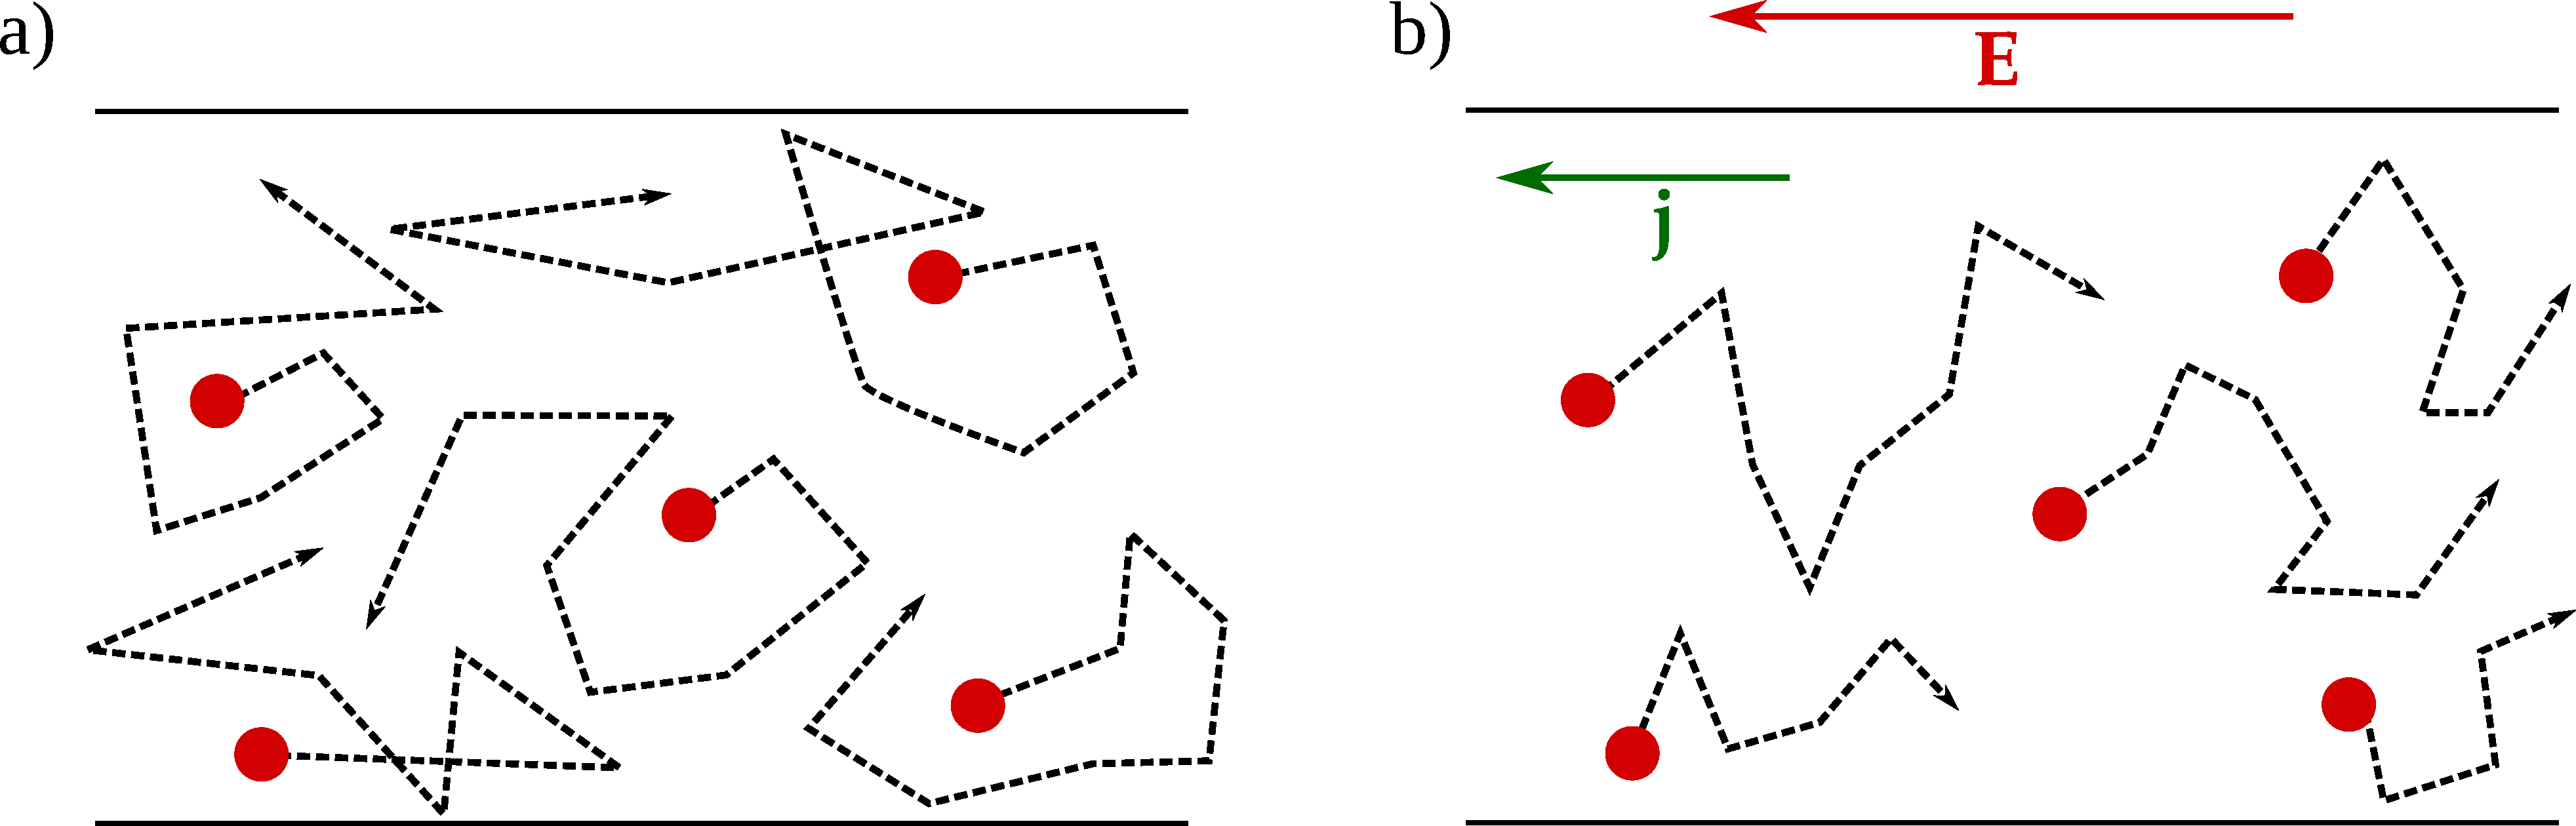
\includegraphics[width=\linewidth]{e_libre}
	\caption{Schéma du mouvement des électrons libres dans un conducteur
		 sans champ électrique (à gauche) et avec champ électrique 
	 	 (à droite). Le champ électrique conduit à un mouvement 
	 	d'ensemble qui génère un vecteur densité de courant $\mitbf{j}$.}%
	\label{fig:e_libre}
\end{figure}

Les conducteurs contiennent des \emph{électrons libres}, c'est-à-dire libres de se 
mouvoir. Ces derniers, soumis à l'agitation thermique, sont animés d'un mouvement
erratique (voir Fig.~\ref{fig:e_libre}). 
Pour générer un courant, il est nécessaire
d'exercer une force sur ces derniers, de manière à créer un \emph{mouvement d'ensemble}.
Dans un circuit électrique par exemple, on impose une différence de potentiel 
entre ses bornes. Les conducteurs solides, tels que le cuivre, contiennent
un nombre important d'atomes, l'étude du mouvement d'un électron, intéragissant
avec chaque atome par interaction coulombienne, devient alors 
difficile.
Dans ce chapitre, nous allons voir comment modéliser le comportement macroscopique 
d'un conducteur soumis à un champ électrique.
\section{Quelques rappels sur le courant électrique}

\begin{defn}[Courant électrique]
Un courant électrique est un mouvement de charges électriques. Il est caractérisé 
par son \emph{intensité}, qui mesure le débit de charges électriques qui traverse
une unité de surface par unité de temps. Elle se mesure en ampères ($\ampere$)
qui correspondent à des $\coulomb \usk \reciprocal \second$ et peut-être 
positive ou négative.
\end{defn}

\begin{exemple}
	Les prises domestiques fournissent un courant dont l'intensité vaut
	$\unit{16}{\ampere}$, voire $\unit{32}{\ampere}$ pour les plaques à induction. 
	Pour une batterie de téléphone, l'intensité vaut
	$\unit{1}{\ampere}$ environ.
\end{exemple}

\begin{defn}[Vecteur densité de courant]
	En tout point de l'espace, un courant électrique est caractérisé par le vecteur 
densité de courant  
	\begin{equation}
		\vecj = n q \vecv,
		\label{eq:jnqv}
	\end{equation}
	où $q$ est la charge d'un porteur de charge ($\coulomb$), $n$ est le
	nombre de charges mobiles par unité de volume ($\rpcubic \meter$) et
	$\vecv$ la vitesse d'un porteur de charge. C'est une grandeur additive.
	L'intensité $\mathrm{d}i$
	qui traverse une surface élémentaire $\ds_P$ centrée sur le point 
	$P$ est donc donnée par 
	\begin{equation}
		\mathrm{d}i = \vecj(P) \cdot \ds_P.
	\end{equation}
	L'intensité totale $I$ traversant une surface macroscopique $\mathcal{S}$
	est donc donnée par 
	\begin{equation}
		I = \iint_\mathcal{S} \vecj(P) \cdot \ds_P.
	\end{equation}
\end{defn}

\begin{exemple}
	On considère un câble de chargeur de téléphone de section $S = \unit{1}
	{\milli \meter \squared}$ alimenté par un courant $I = \unit{1}{\ampere}$.
	Si on suppose que le courant est uniforme à l'intérieur du câble, on a
	$\vecj = I/S = \unit{10^6}{\ampere \usk \meter \rpsquared}$. La partie 
	conductrice du câble est composée principalement de cuivre. Dans le cuivre, 
	les porteurs de charges sont des électrons avec $q = \unit{1.6 \times 10^{-19}
	}{\coulomb}$ et $n \approx \unit{10^{29}}{\rpcubic \meter}$. On peut alors remonter
	à la vitesse de dérive des électrons $v = \unit{60}
	{\micro \meter \usk \reciprocal \second}$
\end{exemple}

Le vecteur densité de courant possède une propriété intéressante en régime 
permanent.
En effet, imaginons le cas d'une sphère contenant une charge $Q$. En régime permanent,
la charge $Q$ contenue dans cette sphère est constante. Le débit total de
charge à travers la sphère est donc nulle. Le vecteur densité de courant est donc 
à flux conservatif.

\begin{defn}[Flux conservatif du vecteur densité de courant]
	En régime permanent, le flux du vecteur densité de courant $\vecj$
	à travers une surface fermée $\mathcal{S}$ est nul
	\begin{equation*}
		\oiint_\mathcal{S} \vecj \cdot \ds = 0.
	\end{equation*}
	$\vecj$ est donc à \textbf{flux conservatif}. Cette égalité peut se traduire
	sous une forme locale
	\begin{equation*}
		\grad \cdot \vecj = 0.
	\end{equation*}
\end{defn}

\begin{rema}
	La loi des n\oe{}uds en électrocinétique découle de la conservativité du
	flux du vecteur densité de courant.
\end{rema}

\section{Le modèle de Drude}
On considère dans cette partie un fil électrique de densité volumique
de porteur de charge $n$. En l'absence de champ électrique, le mouvement
des porteurs de charge est erratique. Leur vitesse est donc nulle en moyenne
et le fil n'est traversé par aucun courant. À l'instant $t=0$, il est plongé dans 
un champ électrique $\vece$ uniforme et constant. Un courant apparaît alors dans 
le fil. Dans cette partie, on cherche
à relier la densité de courant $\vecj$ parcourant le fil et le champ électrique 
$\vece$ imposé.

Expérimentalement, on constate que l'intensité du courant, après une certaine durée,
se stabilise à une valeur constante. 
À partir de l'équation~\ref{eq:jnqv}, on conclut que les 
électrons doivent atteindre une vitesse d'ensemble limite dans le fil. Pour modéliser 
ce comportement et par analogie avec la chute d'un corps, 
le physicien Paul Drude propose l'introduction d'une force de frottement 
qui s'opposerait à la mise en mouvement des électrons. Cette force de 
frottements modélise notamment la présence du réseau cristallin dans lequel évolue 
l'électron. 

On considère alors une particule de charge $q$ et de masse $m$ se déplaçant à la
vitesse $\vecv$.
Dans le référentiel du fil, supposé galiléen, cette particule est soumise à la 
force électrostatique $q\vece$ et à la force de frottement fluide $-\alpha \vecv$, 
où $\alpha$ est le coefficient de frottement (\kilogram \usk \reciprocal \second)
caractéristique du milieu. Pour simplifier le problème, 
on considère que sa vitesse est nulle en 
l'absence de champ électrique. On a donc notamment, $\vecv(t = 0) = \mitbf{0}$.
Le principe fondamental de la dynamique appliqué 
à ce porteur de charge donne

\begin{equation}
	m \dfrac{\mathrm{d}\vecv}{\dt} = q\vece - \alpha\vecv
	\iff \dfrac{d\vecv}{\dt} + \dfrac{\vecv}{\tau} = \dfrac{q\vece}{m},
\end{equation}
où $\tau = m/\alpha$ est homogène à un temps. La solution générale de cette équation
s'écrit

\begin{equation}
	\vecv(t) = \veca \exp\left(-\dfrac{t}{\tau}\right) + \dfrac{q\tau}{m}\vece,
\end{equation}
où $\veca$ est une constante d'intégration. Avec la condition initiale,
$\vecv(t=0) = \mitbf{0}$, on obtient

\begin{equation}
	\vecv(t) = \dfrac{q \tau}{m} 
	           \left[1 - \exp\left(\dfrac{-t}{\tau}\right)\right]\vece.
\end{equation}
$\tau$ apparaît alors comme étant le temps de relaxation de la vitesse du  
porteur de charge. Dès que $t$ est plus grand que quelques $\tau$, 
le porteur de charge a atteint la vitesse limite

\begin{equation}
	\vecv_\mathrm{lim} = \dfrac{q \tau}{m} \vece = \dfrac{q}{\alpha} \vece.
\end{equation}
On peut alors établir une relation directe entre entre la densité volumique
de courant $j$ parcourant le fil et le champ électrique $\vece$ imposé sur ce dernier,
en multipliant cette vitesse par $nq$ (voir Éq.~\ref{eq:jnqv})

\begin{equation}
	\vecj = \dfrac{nq^2\tau}{m} \vece = \gamma \vece,
\end{equation}
où $\gamma$ est la conductivité électrique du matériau. On définit de même
la résistivité $\rho$

\begin{equation}
	\rho = \dfrac{1}{\gamma},
\end{equation}
qui s'exprime en $\ohm \usk \rp \meter$.

\begin{defn}[Loi d'Ohm locale]
	La loi d'Ohm locale est une relation constitutive, elle est donc spécifique
	au conducteur. Elle permet de décrire leur réponse à un champ électrique.
	Un conducteur soumis à un champ électrique $\vece$ est traversé
	par une densité volumique de courant $\vecj$ telle que 
	\begin{equation}
		\vecj = \gamma \vece.
	\end{equation}
	$\gamma$ est la conductivité du conducteur. Elle est caractéristique du
	matériau considéré et s'exprime en siemens par mètre ($\siemens \usk 
	\reciprocal \meter$). Elle mesure la facilité d'un courant à parcourir 
	un matériau. En l'absence de champ électrique, le courant à l'intérieur
	d'un conducteur est donc nul. C'est une grandeur qui dépend de la température. 
	Le tableau~\ref{tab:conductivite} donne la conductivité de matériaux usuels.
\end{defn}

\begin{rema}
	On remarque que le champ électrique est toujours orienté dans la même
	direction que le vecteur de densité volumique de courant.
\end{rema}

\begin{table}
	\centering
	\caption{Ordre de grandeur de conductivités de matériaux usuels. Pour le
		 cuivre et l'eau, les valeurs données sont celles obtenues 
	 	 à température ambiante.}
	\begin{tabular}{l|c}
		\textbf{Matériau} & \textbf{Conductivité électrique} 
		($\siemens \usk \reciprocal \meter$)\\ \hline
		Eau distillée 	 & $1.0 \times 10^{-6}$ à $\unit{300}{\kelvin}$ \\[0.5em]
		Cuivre   & $5.9 \times 10^7$ à $\unit{300}{\kelvin}$\\[0.5em]
		Basalte   & $10^{-5} - 0.5$ \\[0.5em]
		Grès     & $10^{-3} - 1$\\[0.5em]
		Argile   & $10^{-2} - 1$\\[0.5em]
		Graphite & $5 \times 10^{2} - 10^4$\\ \hline
	\end{tabular}
	\label{tab:conductivite}
\end{table}

\section{Sondage résistif}
La notion de résistivité est particulièrement intéressante en sciences de la 
Terre. Elle est notamment utilisée pour sonder le sol à la recherche de minerai.
Comme le montre le Tableau~\ref{tab:conductivite}, la résistivité des minerais tels que
le cuivre est bien plus élevée que celle des roches qui le contiennent. Ce contraste
de résistivité permet alors de les localiser en utilisant par exemple le montage
à 4 électrodes que nous allons présenter.

\subsection{Potentiel électrique d'une électrode}
\begin{figure}[]
	\centering
	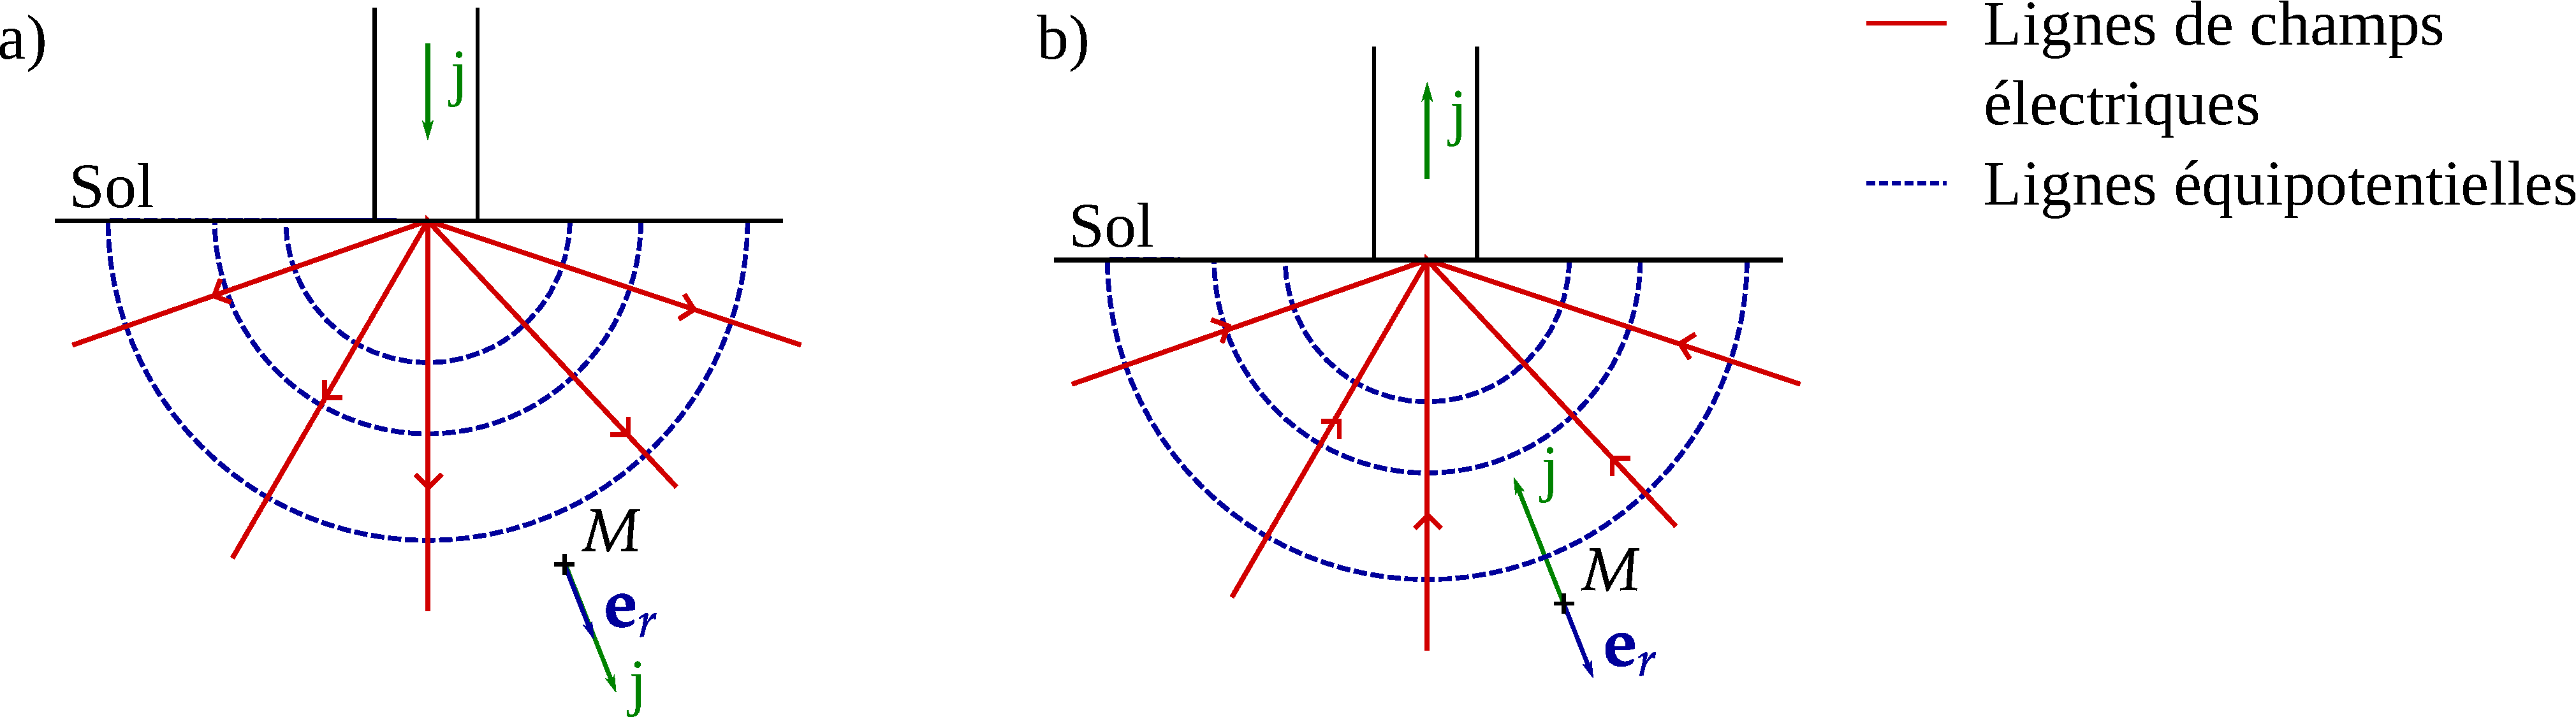
\includegraphics[scale=1]{electrode}
	\caption{Schéma d'une électrode émettrice (à gauche) et réceptrice (à droite).
		 L'électrode est parcourue
	par une densité volumique de courant $\vecj$. Elle génère dans le sol
	un champ électrique $\vece$ dont on a représenté les lignes de champs en rouge.
	Quelques lignes équipotentielles du potentiel $V$ résultant de ce champ
	sont dessinées sous la forme de lignes bleues pointillées.}%
	\label{fig:electrode}
\end{figure}

On considère une électrode de section $S$ parcourue par un courant d'intensité $I$ 
et de densité volumique de courant $\vecj$ plantée dans un sol uniforme de résistivité
$\rho$. (voir Fig~\ref{fig:electrode}a). Le point de contact de l'électrode avec le sol
agit comme une source de courant en injectant un courant d'intensité $I$ dans
ce dernier. Le système présente une symétrie sphérique, $\vecj$ ne dépend donc 
que de la distance à l'électrode et est porté par le vecteur radial $\er$.
La densité de courant volumique $\vecj$ en un point $M$ de l'espace à une
distance $r$ de la source est donnée par

\begin{equation}
	\vecj(r) = \dfrac{I}{2 \pi r^2} \er,
\end{equation}
où $2 \pi r^2$ est la surface de la demi-sphère de rayon $r$.
Cette électrode génère donc dans le sol un champ électrique $\vece$ relié
à $\vecj$ par la loi d'Ohm locale

\begin{equation}
	\vece(r) = \rho \vecj(r) = \dfrac{\rho I}{2 \pi r^2} \er.
\end{equation}
Le potentiel électrostatique $V$ en un point $M$ de l'espace est donc déduit
en utilisant la relation liant le champ électrique au potentiel électrostatique

\begin{equation}
	\vece (r) = -\grad(V) = -\dfrac{\mathrm{d}V}{\dr}(r) \er 
	\iff V(r) = \dfrac{\rho I}{2 \pi r}
	\label{eq:potentiel}
\end{equation}
en fixant le potentiel électrostatique nul en l'infini.
Le potentiel électrostatique dépend donc directement de la résistivité du milieu
considéré.

\subsection{Le montage à 4 électrodes}
\begin{figure}[]
	\centering
	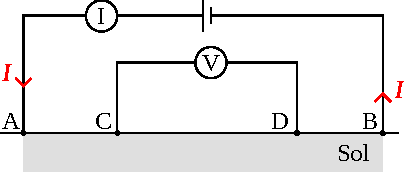
\includegraphics[]{4electrode}
	\caption{Schéma du montage à 4 électrodes. Le générateur fournit un courant
		 d'intensité $I$ qui se distribue dans le sol en A et ressurgit en 
	 	 B. Un voltmètre et un ampèremètre permettent de mesurer respectivement
		 la tension
	 	 entre les points D et C et l'intensité $I$. Les électrode D
	 	 et C ne sont parcourues par aucun courant.}%
	\label{fig:4electrode}
\end{figure}
On présente maintenant le montage à 4 électrodes qui permet de remonter à la 
résistivité $\rho$ du sol. On considère ici un sol uniforme.
La Figure~\ref{fig:4electrode} fourni un schéma 
du montage. D'après l'équation~\ref{eq:potentiel}, les électrodes en A et B 
génèrent un potentiel en C donné par
\begin{equation*}
	V_C^A = \dfrac{\rho I}{2 \pi |AC|} \quad \mathrm{et} \quad
	V_C^B = -\dfrac{\rho I}{2 \pi |BC|}.
\end{equation*}
Le signe $-$ dans l'expression de $V_C^B$ provient de l'orientation de $\vecj$ 
au point D (voir Fig.~\ref{fig:electrode}b). Finalement, le potentiel au point $C$
résulte de la superposition de ces deux potentiels
\begin{equation*}
	V_C = V_C^A + V_C^B = \dfrac{\rho I}{2 \pi}
	                    \left(\dfrac{1}{|AC|} - \dfrac{1}{|BC|}\right).
\end{equation*}
De même, le potentiel de l'électrode au point D est donnée par
\begin{equation*}
	V_D = \dfrac{\rho I}{2 \pi}
	      \left(\dfrac{1}{|AD|} - \dfrac{1}{|BD|}\right).
\end{equation*}
La différence de potentiel $\Delta V$mesurée par le voltmètre est donc donnée par 
\begin{equation*}
	\Delta V = V_C - V_D = \dfrac{\rho I}{2 \pi}\left(
		\dfrac{1}{|AC|} - \dfrac{1}{|BC|}
	- \dfrac{1}{|AD|} + \dfrac{1}{|BD|} \right)
\end{equation*}
En dehors de la résistivité $\rho$, toutes les autres grandeurs apparaissant dans
cette égalité sont connues. On peut donc remonter à la résistivité du sol
\begin{equation}
	\rho = \dfrac{2 \pi \Delta V}{I}\left(
		\dfrac{1}{|AC|} - \dfrac{1}{|BC|}
	- \dfrac{1}{|AD|} + \dfrac{1}{|BD|} \right)^{-1}
\end{equation}
Certaines configurations d'électrodes permettent d'obtenir une formule finale
simple. On peut citer par exemple la configuration de Wenner, pour laquelle
$|AC| = |DB| = a$ et $|CB| = |AD| = 2a$. La formule précédente devient alors
\begin{equation}
	\rho = 2 \pi a \dfrac{V}{I}.
\end{equation}

\subsection{Distribution de courant}
\begin{figure}[]
	\centering
	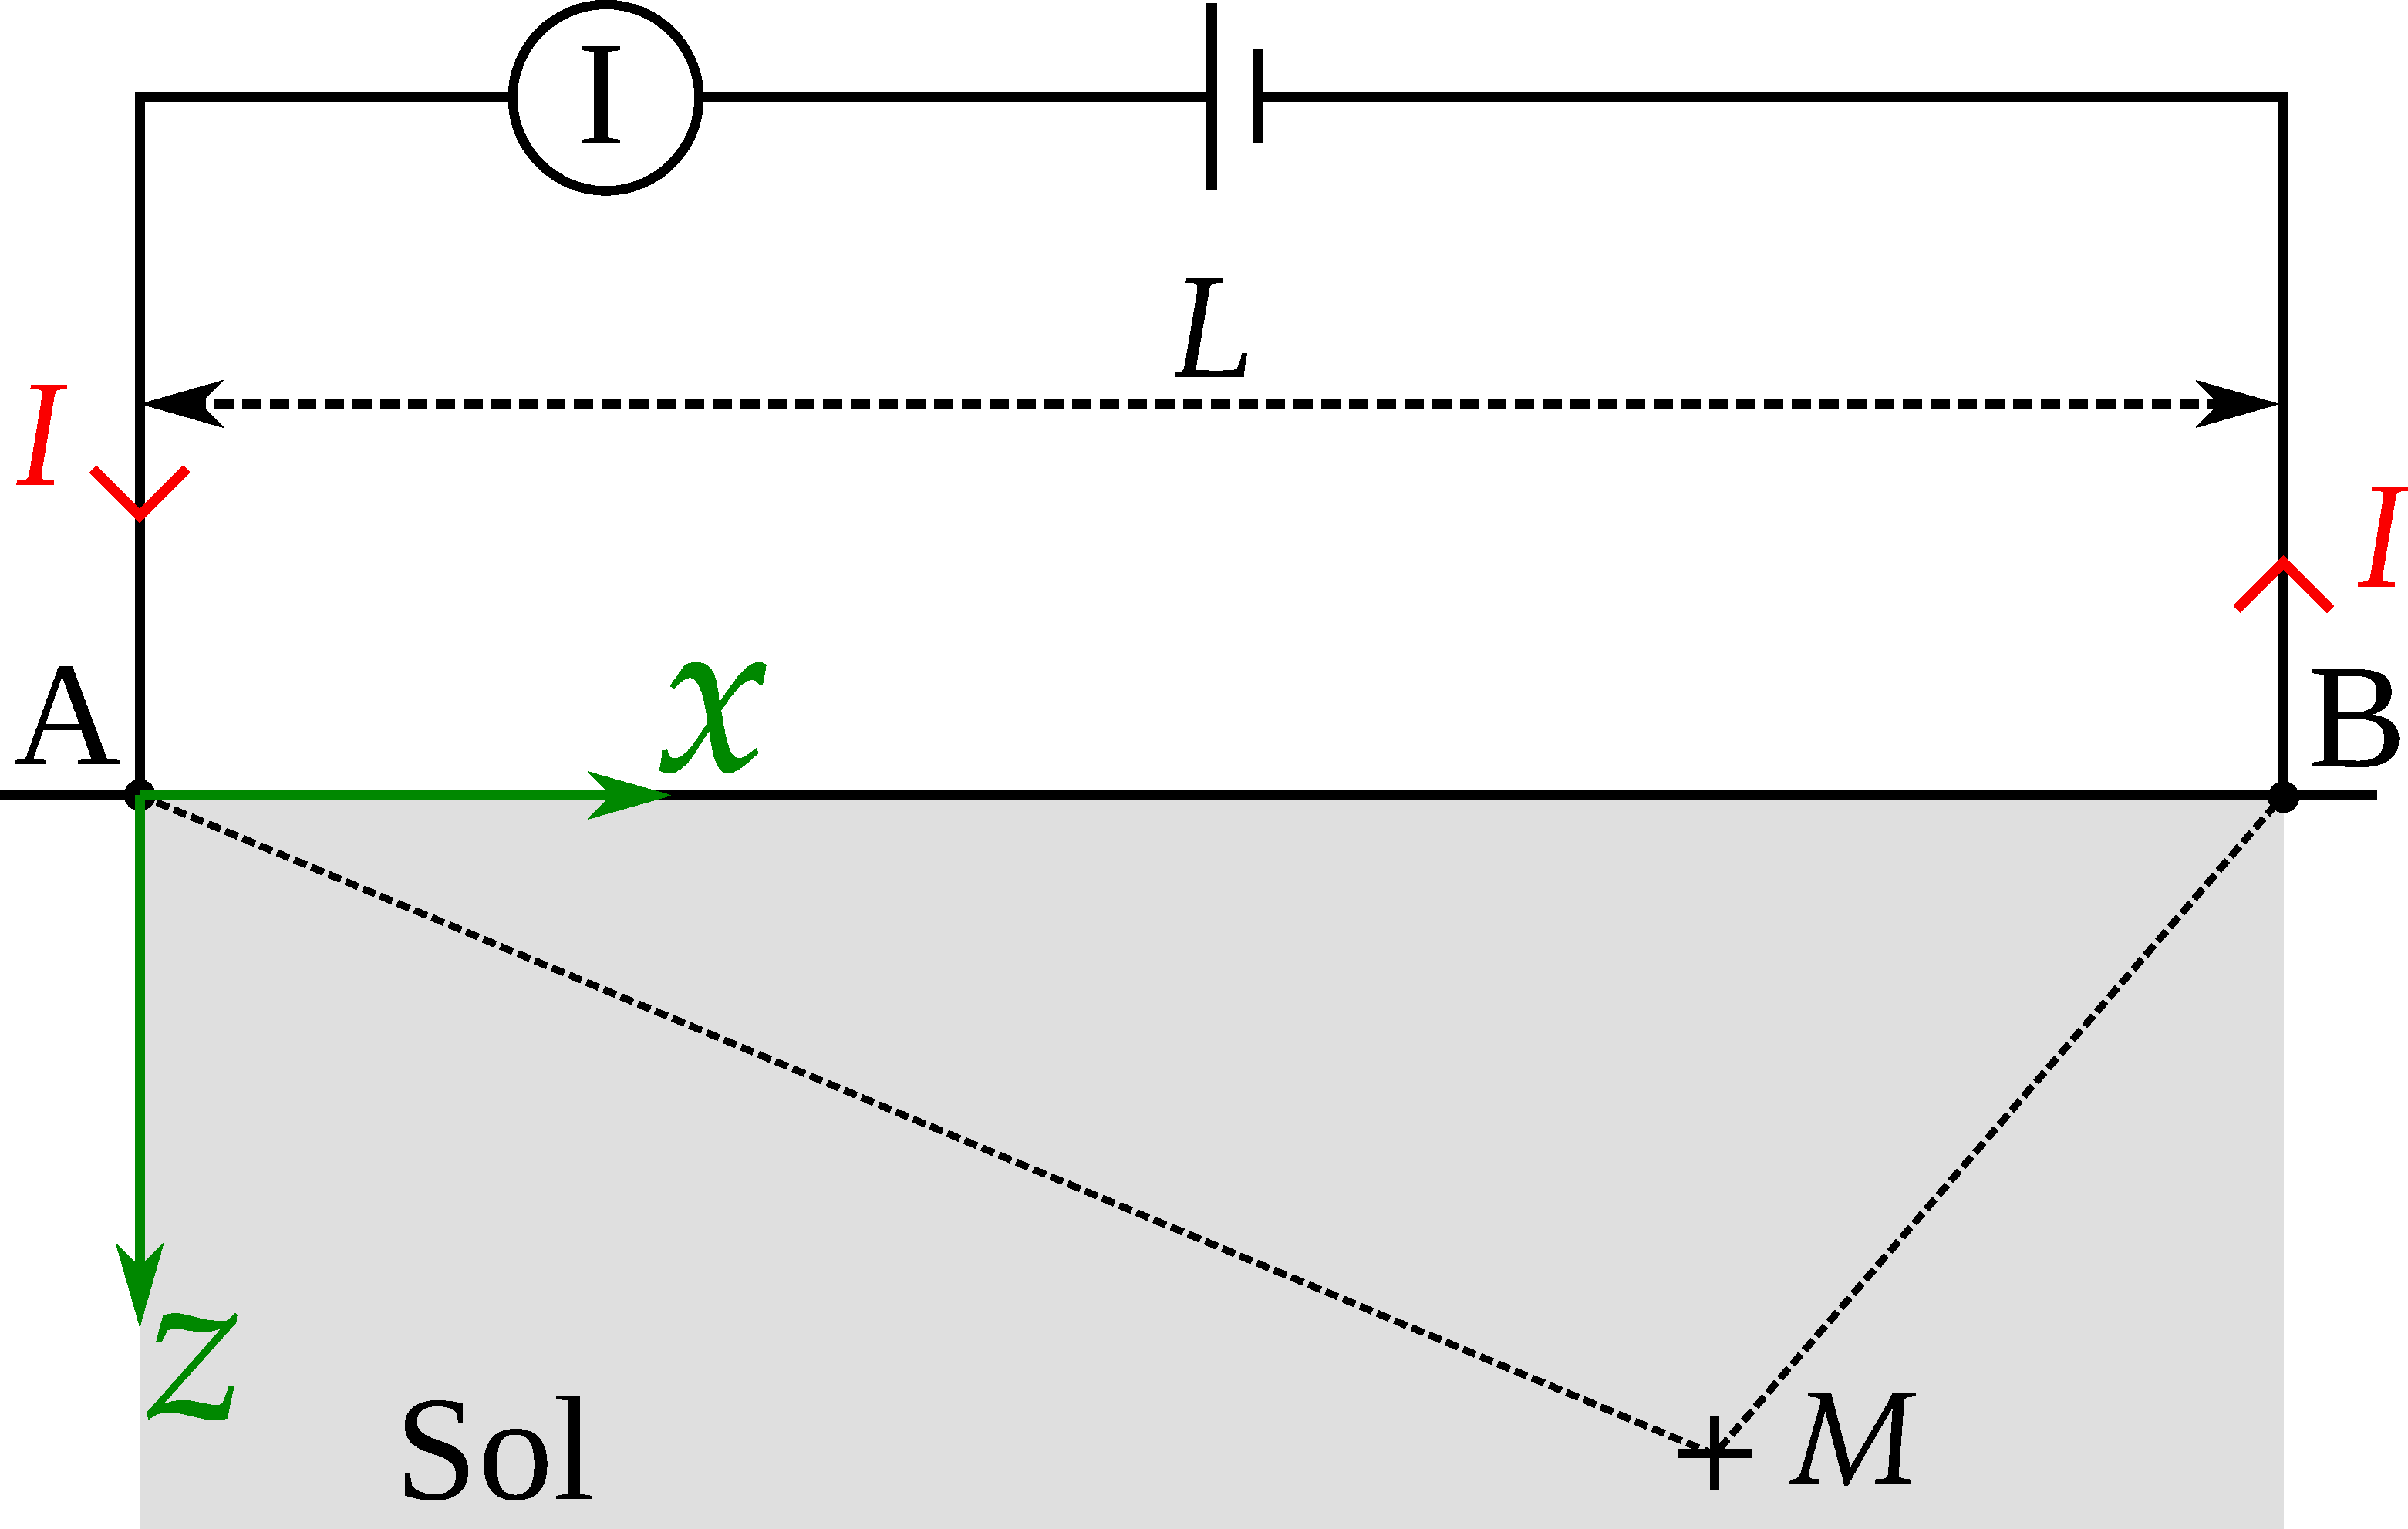
\includegraphics[]{penetration_courant}
	\caption{Paire d'électrodes alimentées par un courant d'intensité $I$
		 et séparées par une distance $L$.}%
	\label{fig:penetration_courant}
\end{figure}
On s'intéresse maintenant à la distribution de courant générée dans le sol
par une paire d'électrodes émettrice-réceptrice. On cherche à connaître la 
profondeur maximale que permet de sonder une paire d'électrodes. 

On considère donc une paire d'électrodes A et B alimentées par un courant d'
intensité $I$ et séparées 
par une distance $L$ (voir Fig.~\ref{fig:penetration_courant}). 
Le sol est un demi-espace infini de résistivité $\rho$ uniforme. 
On se place dans un repère cartésien $(O, \ex, \ey, \ez)$. Un point $M$ de l'espace
est donc repéré par ses coordonnées $(x, y, z)$.

La paire d'électrodes génère au point $M$ un champ électrostatique $\vece$ dont
la composante selon $\ex$ vaut
\begin{equation*}
	E_x(M) = - \dfrac{\partial}{\ddx}\left[\dfrac{\rho I}{2 \pi} 
	\left( \dfrac{1}{|AM|} - \dfrac{1}{|BM|}\right)\right],
\end{equation*}
où $|AM| = \sqrt{x^2 + y^2 + z^2}$ et $|BM| = \sqrt{(L - x)^2 + y^2 + z^2}$.
On a alors
\begin{equation*}
	E_x(M) = \dfrac{\rho I}{2 \pi}\left(\dfrac{x}{|AM|^3} 
	    + \dfrac{L - x}{|BM|^3}\right).
\end{equation*}
On peut alors aboutir à la composante $j_x$ de la densité volumique de courant
$\vecj$ en utilisant la loi d'Ohm
\begin{equation}
	j_x(M) = \dfrac{E_x}{\rho} = \dfrac{I}{2 \pi}\left(\dfrac{x}{|AM|^3} 
	    + \dfrac{L - x}{|BM|^3}\right).
\end{equation}

\begin{figure}[]
	\centering
	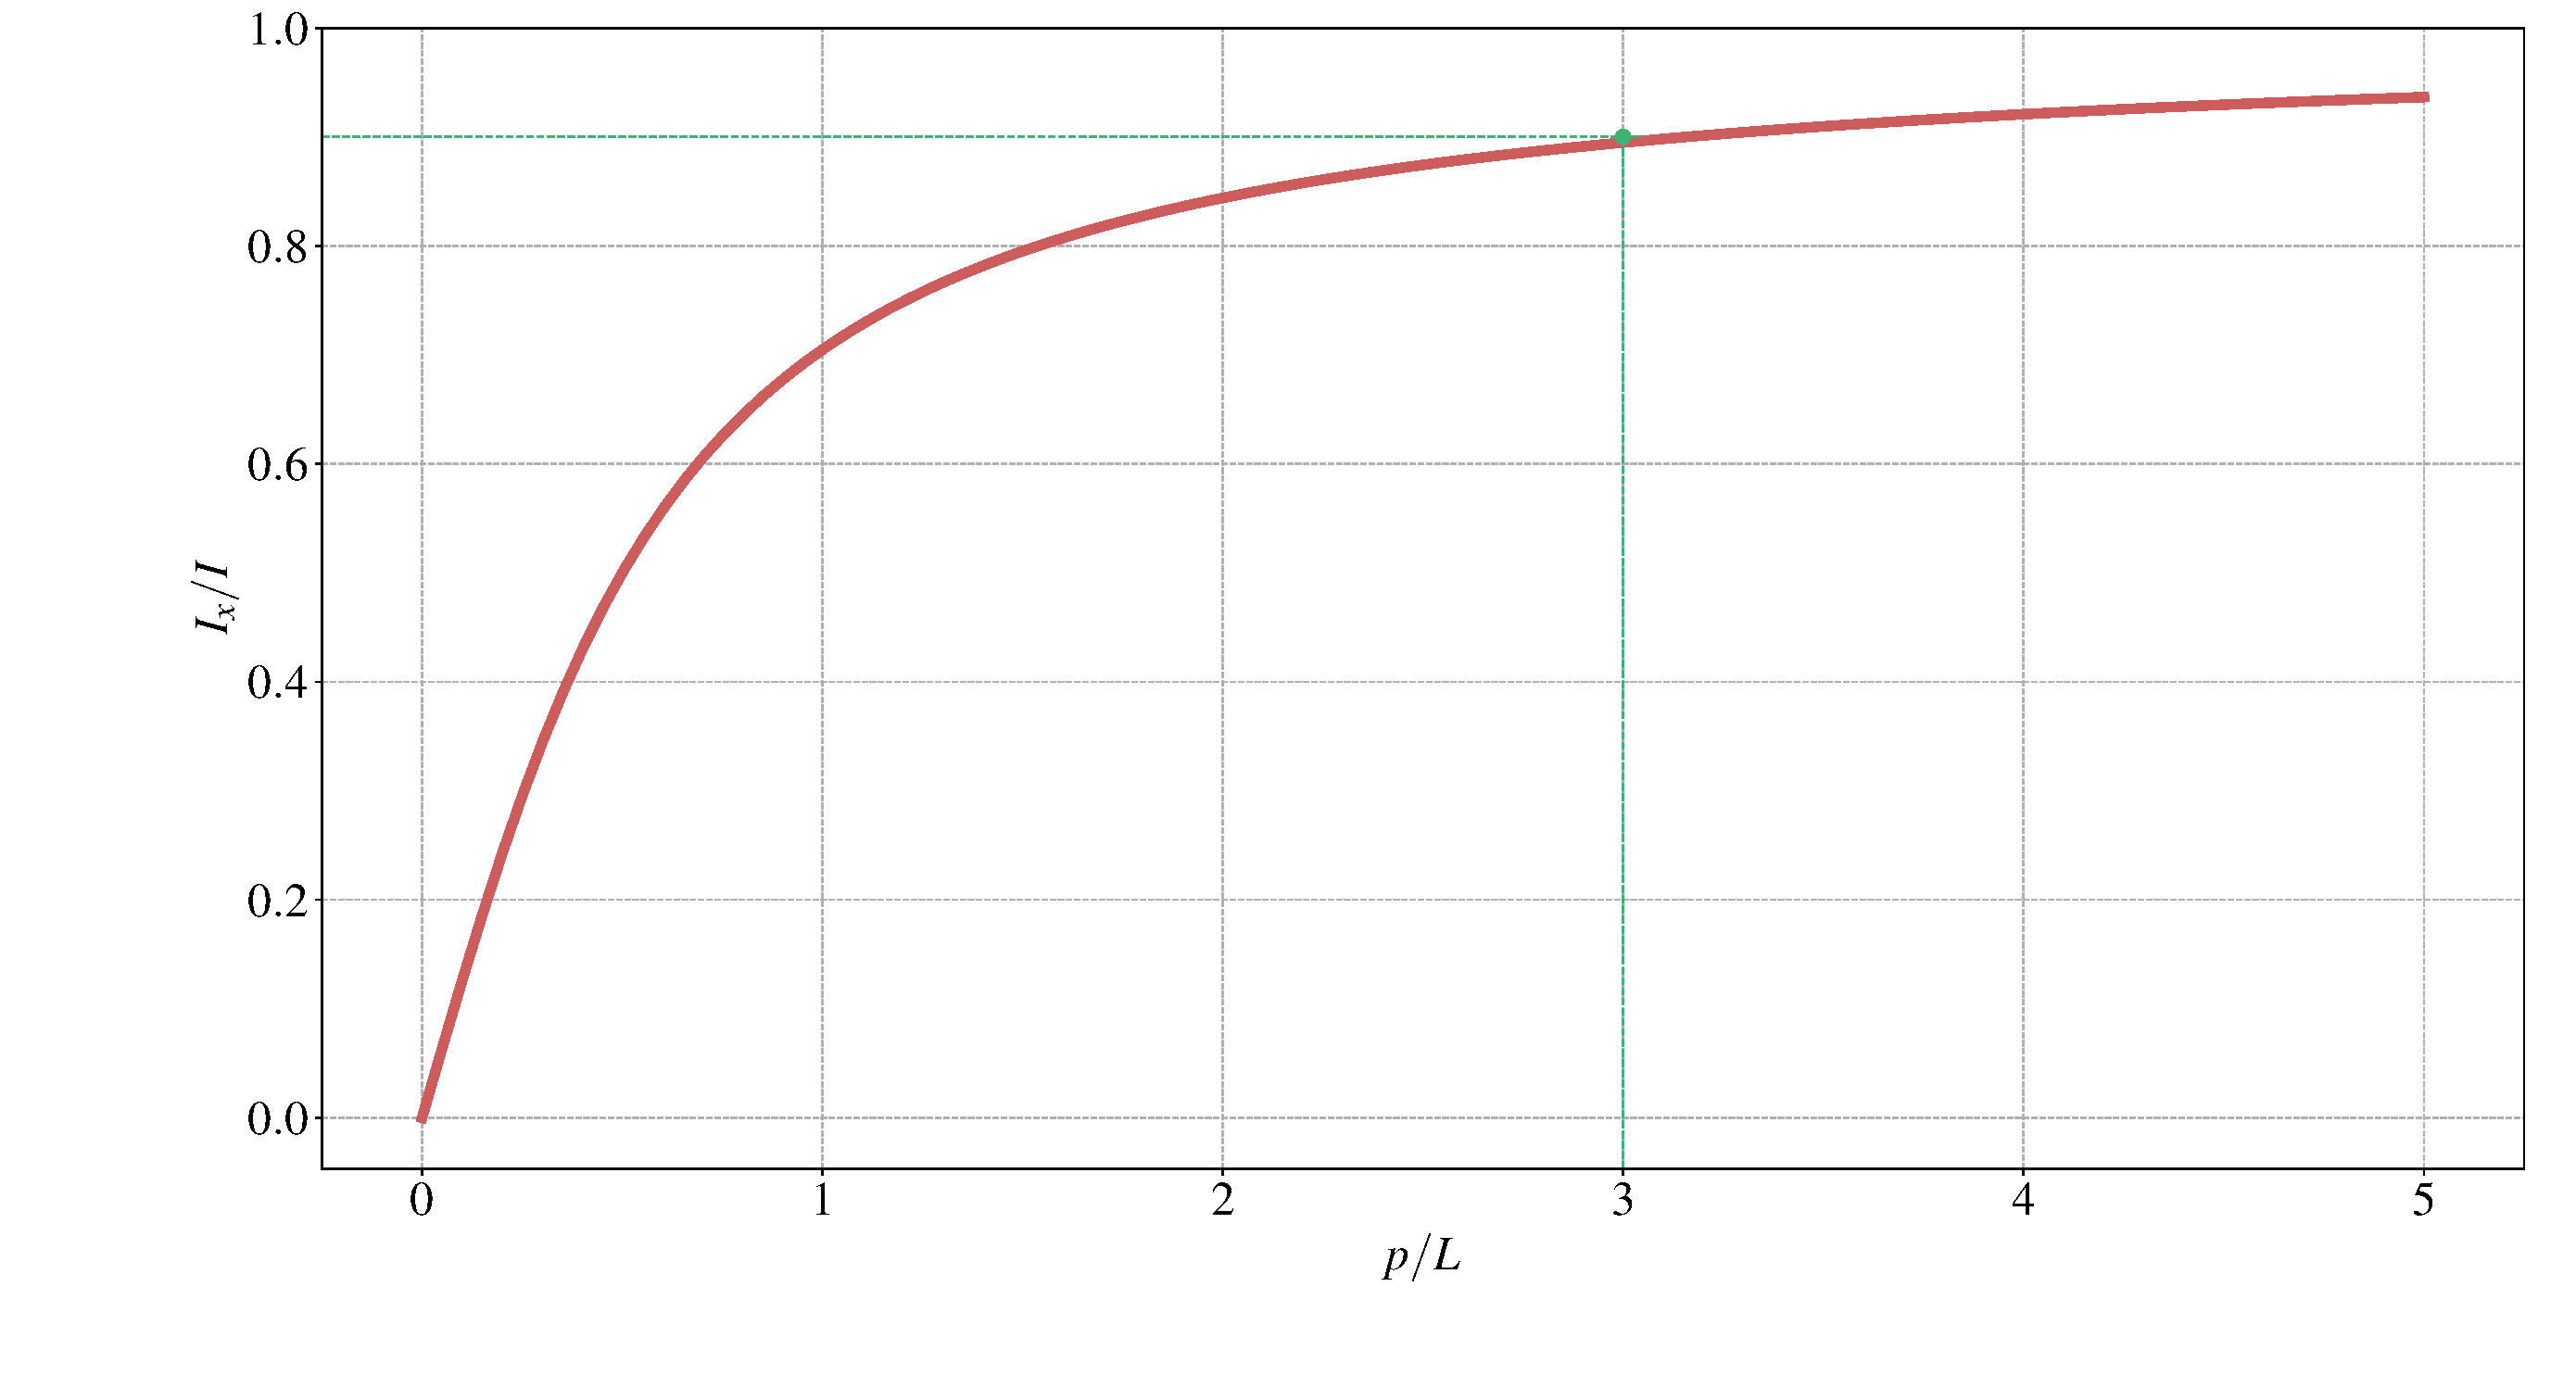
\includegraphics[scale=0.8]{arctan}
	\caption{Intensité relative traversant une section de sol située 
		en $x = L/2$ jusqu'à la profondeur
	$p$ en fonction du rapport de $p$ sur la distance inter-électrode $L$.
	Le point vert correspond au point particulier $(3, 0.9)$.}%
	\label{fig:arctan}
\end{figure}

On s'intéresse maintenant au cas où le point $M$ appartient au plan médian $
x = L/2$ aux
deux électrodes. Dans ce cas particulier, $j_x$ vaut
\begin{equation*}
	j_x(M) = \dfrac{IL}{2 \pi \left[(L/2)^2 + y^2 + z^2\right]^{3/2}}.
\end{equation*}
L'intensité $\mathrm{d}I_x$ du courant traversant la surface 
élémentaire $\dy\dz \ex$ centré en $M$ s'écrit
\begin{equation*}
	\mathrm{d}I_x = \vecj(M) \cdot \dy\dz\ex = j_x(M) \dy\dz
	    = \dfrac{IL}{2 \pi \left[(L/2)^2 + y^2 + z^2\right]^{3/2}} \dy\dz.
\end{equation*}
La fraction de courant qui traverse une section du plan médian jusqu'à une 
profondeur $p$ est alors donnée par
\begin{equation*}
	\dfrac{I_x}{I}(p) = \int_{y=-\infty}^{y=\infty} \int_{z=0}^{z=p}
	\dfrac{IL}{2 \pi \left[(L/2)^2 + y^2 + z^2\right]^{3/2}} \dy\dz.
\end{equation*}
Comme 
	\begin{equation*}
		\int_{y=-\infty}^{y=\infty} \dfrac{\dy}{
			\left[(L/2)^2 + y^2 + z^2\right]^{3/2}} = 
		\dfrac{2}{\left[(L/2)^2 + z^2\right]^{3/2}},
	\end{equation*}
l'équation précédente devient
\begin{equation*}
	\dfrac{I_x}{I}(p) = \int_{z=0}^{z=p}
	\dfrac{IL}{\pi \left[(L/2)^2 + z^2\right]} \dz.
\end{equation*}
On obtient alors finalement
\begin{equation}
	\dfrac{I_x}{I}(p) = \dfrac{2}{\pi}\arctan\left(\dfrac{2p}{L}\right).
\end{equation}

Sur la Figure~\ref{fig:arctan}, on a tracé l'évolution de l'intensité relative traversant
une section de sol située en $x = L/2$ 
jusqu'à la profondeur $p$ en fonction du rapport de $p$ sur 
la distance inter-électrode $L$. 
On remarque que $90\,\%$ de l'intensité $I$ traverse une section de sol s'étendant
jusqu'à la profondeur $3L$. En augmentant la distance $L$ entre les deux électrodes,
on peut alors sonder le sol à une profondeur plus élevée.

\subsection{Résistivité apparente}
\begin{figure}[t]
	\centering
	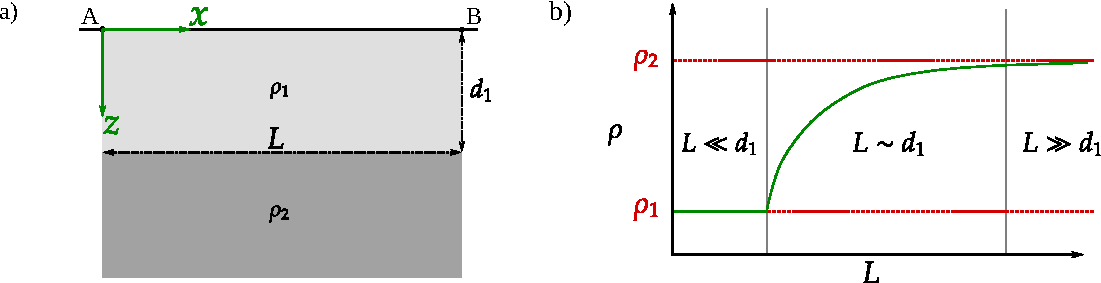
\includegraphics[scale=0.8]{resistivite_apparente}
	\caption{Mesure de la résistivité d'un sol bicouche avec 2 électrodes
		avec le montage à gauche et l'évolution schématique de la résistivité
		apparente $\rho$ avec la distance $L$ entre les électrodes à droite.
		Les deux électrodes sont séparées d'une distance $L$ et 
		alimentées par un courant d'intensité $I$. La première couche 
		présente une épaisseur $d_1$ et une résistivité $\rho_1$, tandis
		que la seconde couche présente une résistivité 
		$\rho_2$ avec $\rho_1 < \rho_2$.}%
	\label{fig:apparente}
\end{figure}

Nous n'avons pour l'instant considéré que le cas idéal d'un sol de résistivité 
uniforme $\rho$. Dans ce cas bien précis, la méthode des 4 électrodes permet de
déterminer la résistivité exacte de ce dernier. 

En réalité, la résistivité d'un sol est une fonction complexe de l'espace qui résulte 
de sa composition, de sa température et d'autres paramètres physiques. 
La résistivité mesurée par la méthode des 4 électrodes est alors
qualifiée d'\emph{apparente}. Cette mesure donne néanmoins des informations utiles
sur la structure du sol sondé.

Pour bien illustrer cela, on considère le cas d'un sol composé de deux couches
de résistivités uniformes $\rho_1$ et $\rho_2$, avec $\rho_2 > \rho_1$. La couche $1$ 
s'étend sur une épaisseur $d_1$ (voir Fig.~\ref{fig:apparente}(a)). 
Pour simplifier le problème,
on décide de sonder ce sol à l'aide de deux électrodes séparées d'une distance $L$
et alimentées par un courant d'intensité $I$. La résistivité mesurée va alors dépendre de
la distance entre les deux électrodes (voir Fig.~\ref{fig:apparente}(b))
\begin{enumerate}
	\item lorsque $L \ll d_1$, seule la première couche de sol est sondée.
	  La résistivité mesurée sera alors proche de $\rho_1$.
	\item lorsque $L \gg d_1$, la majeure partie de l'intensité traverse la seconde
	  couche de sol. La résistivité mesurée tend vers $\rho_2$.
	\item lorsque $L \sim d_1$, les deux couches sont sondées de manière équivalente.
	  La résistivité mesurée se situe entre $\rho_1$ et $\rho_2$.
\end{enumerate}
En faisant varier la distance $L$ entre les deux électrodes, on est alors capable d'avoir
une carte schématique de la résistivité du sol sondé et donc de connaître la 
composition de ce dernier. 


